\section{Fair Atomic Swaps}
\label{sec:fair_atomic_swap}

In this section, we propose an improvement on the original Atomic Swap to make it fair.
It implements the premium mechanism, and supports both the currency exchange-style Atomic Swap and the American Call Option-style Atomic Swap.


\subsection{Design}

\subsubsection{Difference between Currency Exchange and Options}
\label{subsubsec:diff_spot_option}

We first summarise the design objectives for Atomic Swap.

To our knowledge, the Atomic Swap protocol is originally designed for the fair exchange between different cryptocurrencies.
However, according to our analysis, the protocol is unfair due to the Optionality and the free premium.
Also, for (crypto)currency exchange, the protocol should have no Optionality.
The currency exchange and the American Call Option differ in Finance: the currency exchange is a type of Spots~\cite{hull1991introduction}, while the American Call Option is a type of Options.
The Spot Contract and the Option Contract aim at different application scenarios: the Spot Contract aims at exchanging the ownership of assets, while the Option Contract aims at providing Alice an ``option'' to trade.
More specifically, Spots and Options differ in the following aspects:

\begin{itemize}
    \item The Spot Contract is exercised immediately, while the Option Contract is exercised on or prior to a specified date in the future.
    \item The Spot Contract cannot be aborted once signed by both parties, while in the Option Contract Alice can abort the contract with the loss of the premium.
    \item The Spot Contract itself has no value, while the Option Contract itself has value - the premium.
\end{itemize}

\subsubsection{Premium for Currency Exchange and American Call Options}
\label{subsubsec:design_obj}

According to Section~\ref{subsubsec:diff_spot_option}, the currency exchange-style Atomic Swaps and the American Call Option-style Atomic Swaps differ in design objectives.

\paragraph{Atomic Swaps for Currency Exchange}
For the currency exchange, both parties are not permitted to abort the contract once signed.
However, in Atomic Swaps, Alice can abort the swap by not releasing the random secret.
Therefore, the protocol should discourage Alice to abort the swap.
To achieve this, we can use the premium mechanism as the collateral: Alice should deposit the premium besides her asset when \textbf{Initiate}.
The premium should follow that:
\textbf{Alice pays the premium to Bob if Bob refunds his asset after his timelock but before Alice's timelock.
If Alice's timelock expires, Alice can refund her premium back.}

\paragraph{Atomic Swaps for American Call Options}
For the American Call Options, Alice should pay for the premium besides the underlying asset, regardless of whether the swap is successful or not.
In reality, the option sellers are trustworthy - the option sellers never abort the contract.
However, in Atomic Swaps, Bob can abort the contracts like Alice.
To keep the Atomic Swap consistent with the American Call Options,
the premium should follow that: 
\textbf{Alice pays the premium to Bob if
1) Alice redeems Bob's asset before Bob's timelock, or
2) Bob refunds his asset after Bob's timelock but before Alice's timelock.
If Alice's timelock expires, Alice can refund her premium back.}











\subsection{Our protocol}


\begin{figure}[htp]
    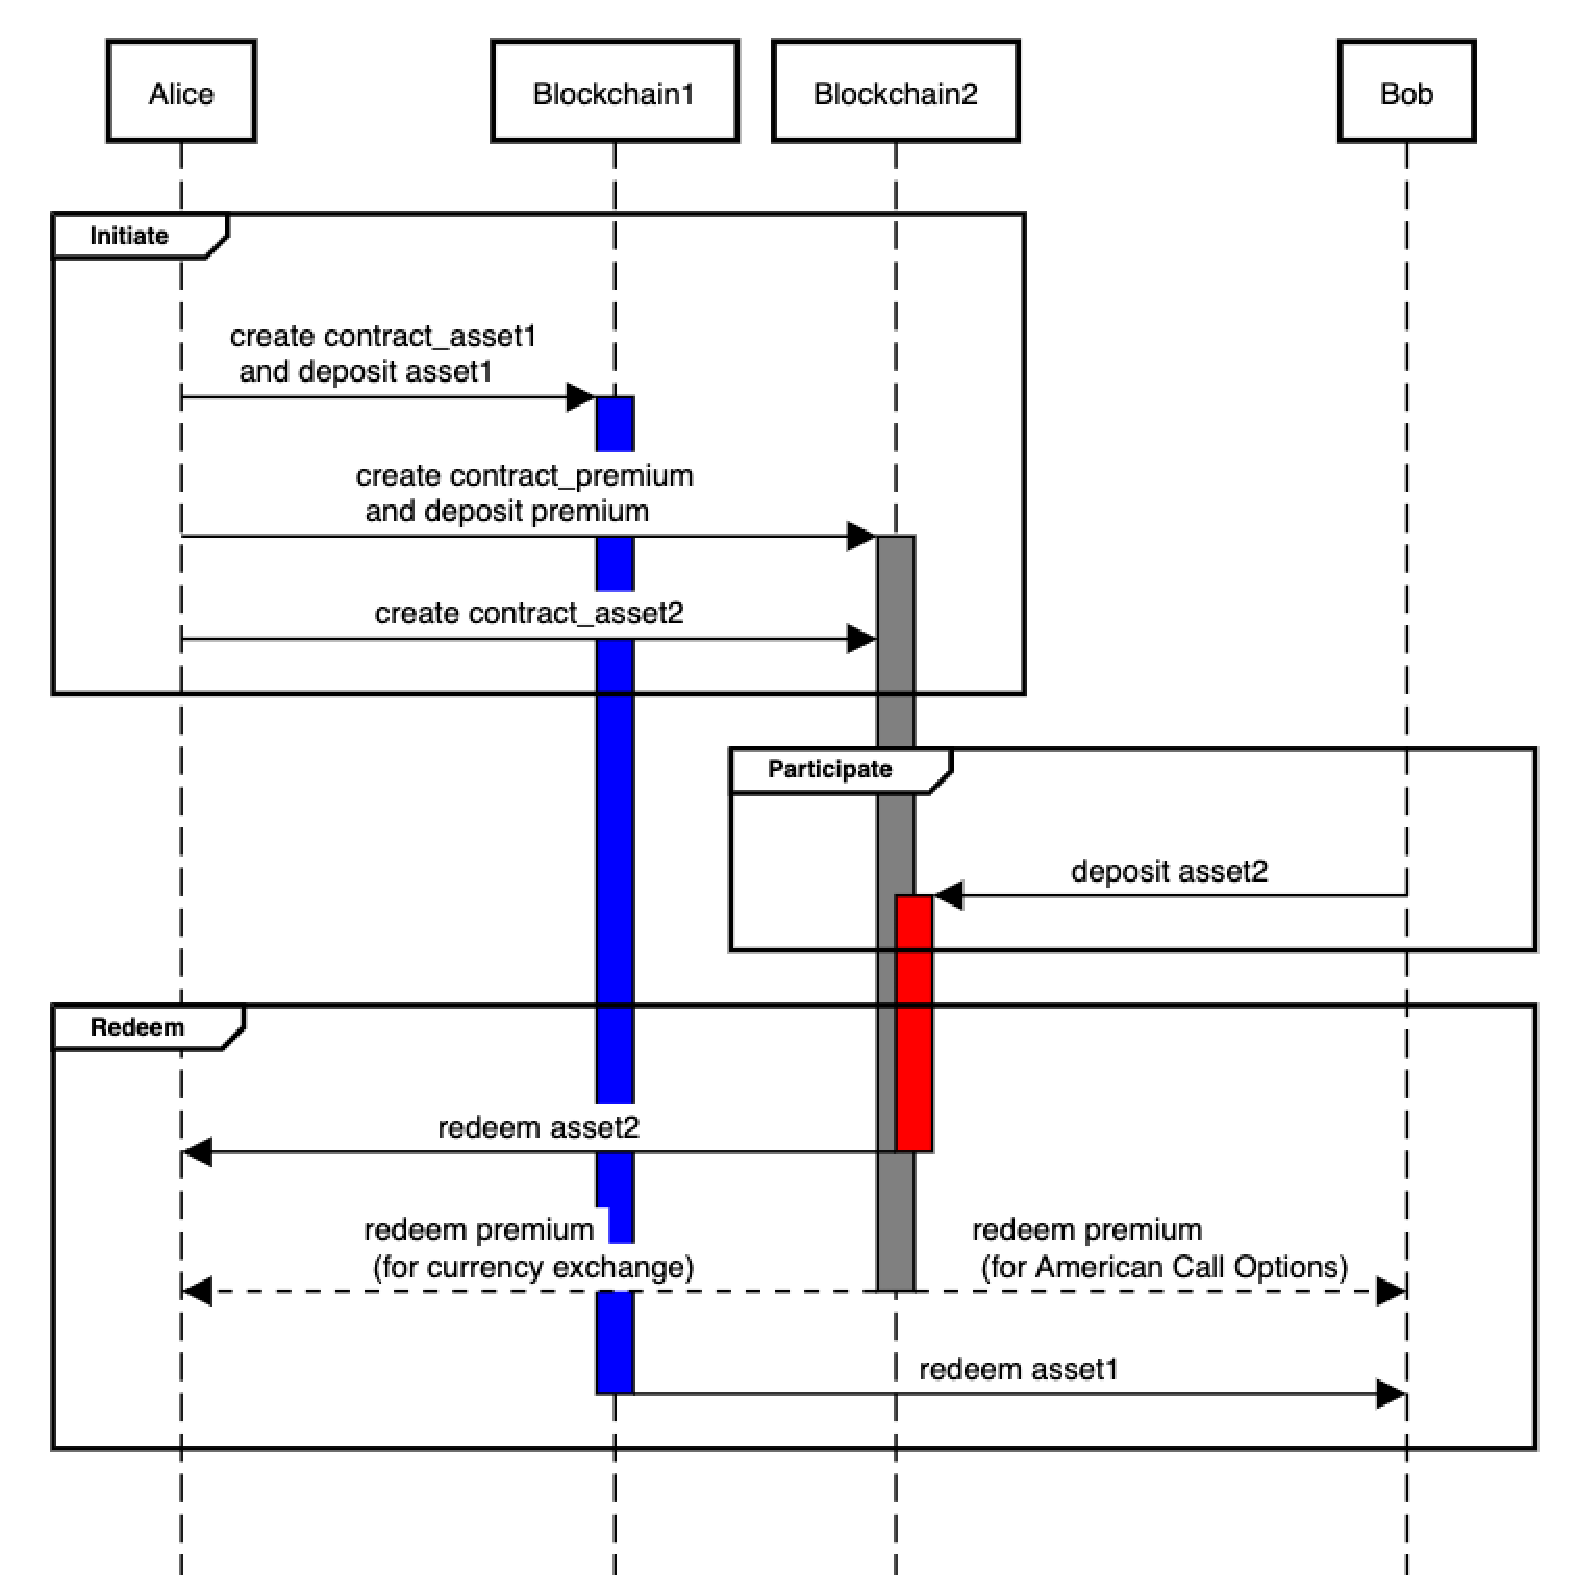
\includegraphics[width=.9\linewidth]{sequence_diagram_us.eps}
    \caption{Sequence diagram of our Atomic Swap.
    For currency exchange-style Atomic Swaps, the premium will go back to Alice if the swap is successful (the left dotted line).
    For American Call Option-style Atomic Swaps, the premium will go to Bob if the swap is successful (the right dotted line).}
    \label{fig:sequence_diagram_us}
\end{figure}

We propose an improvement on the Atomic Swap, which implements the premium mechanism, to make it fair.
It can fulfill design objectives of both the currency exchange and the American Call Option.
Figure~\ref{fig:sequence_diagram_us}) shows the process of our Atomic Swap.

We denote our Atomic Swap protocol $\mathcal{AS}'$ as

$$\mathcal{AS}' = (x_1, Coin_1, x_2, Coin_2, pr)$$

where $pr$ is the amount of the premium measured in $Coin_2$.
In our protocol, besides $x_1$ $Coin_1$, Alice should also lock $pr$ $Coin_2$ on $BC_2$, which will be described later.

Similar to the original Atomic Swap $\mathcal{AS}$, our protocol consists of four stages:
\textbf{Initiate}, \textbf{Participate}, \textbf{Redeem} and \textbf{Refund}.

\paragraph{\textbf{Initiate}}
Different from $\mathcal{AS}$, Alice also creates Bob's contract script $\mathcal{C}_2$ and its associated transaction $tx_{\mathcal{C}, 2}$ when \textbf{Initiate} in $\mathcal{AS}'$.

$\mathcal{C}_1$ and $tx_{\mathcal{C}, 1}$ is the same as in $\mathcal{AS}$,
while $\mathcal{C}_2$ and $tx_{\mathcal{C}, 2}$ are more sophisticated.
$\mathcal{C}_2$ contains two coherent sub-contracts $\mathcal{C}^{asset}_2$ and $\mathcal{C}^{pr}_2$.

In $\mathcal{C}_2$, $\mathcal{C}^{asset}_2$ is the contract for the asset $x_2$ $Coin_2$, which is the same as in $\mathcal{AS}$.
$\mathcal{C}^{pr}_2$ is the contract for the premium $pr$, which implements the premium mechanism in the Atomic Swap.
It supports both the currency exchange-style Atomic Swap and the American Call Option-style Atomic Swap.
In more detail, the rules of $\mathcal{C}^{pr}_2$ are shown below:

\begin{description}
    \item[$\mathcal{C}^{pr}_2$ for currency exchange] Alice pays $pr$ to Bob with the condition:
    Bob refunds $x_2$ $Coin_2$ after $\delta_2$ and before $\delta_1$.
    If $\delta_1$ expires, Alice can refund $pr$ back.
    \item[$\mathcal{C}^{pr}_2$ for American Call Options] Alice pays $pr$ to Bob with one of the two conditions:
    1) Alice redeems $x_2$ $Coin_2$ before $\delta_2$.
    2) Bob refunds $x_2$ $Coin_2$ after $\delta_2$ but before $Delta_1$ (note that $\delta_2 < \delta_1$).
    If $\delta_1$ expires, Alice can refund $pr$ back.
\end{description}

Alice published $tx_{\mathcal{C}, 1}$ on $BC_1$ and $tx_{\mathcal{C}, 2}$ on $BC_2$.
Note that Alice only triggers $\mathcal{C}_1$ and $\mathcal{C}^{pr}_2$ to execute at this stage.
Bob will deposit $x_2$ $Coin_2$ trigger $\mathcal{C}^{asset}_2$ to execute when \textbf{Participate}.

\paragraph{\textbf{Participate}}
Bob decides whether to participate in $\mathcal{AS}'$ by auditing $tx_{\mathcal{C}, 1}$ and $tx_{\mathcal{C}, 2}$.
If Bob thinks contracts are fair, he will participate in $\mathcal{AS}'$, otherwise Bob will not participate and look for more profitable contracts from others.
To participate in $\mathcal{AS}'$, Bob deposits $x_2$ $Coin_2$ in $\mathcal{C}^{asset}_2$, and triggers $\mathcal{C}^{asset}_2$ to execute.

\paragraph{\textbf{Redeem}}
Alice redeeming $x_2$ $Coin_2$ and Bob redeeming $x_1$ $Coin_1$ are the same in $\mathcal{AS}'$ and $\mathcal{AS}$.
But in addition, riles in $\mathcal{C}^{pr}_2$ will work once triggering \textbf{Redeem} for $\mathcal{AS}'$.

\paragraph{\textbf{Refund}}
Refunding $x_1$ $Coin_1$ for Alice and $x_2$ $Coin_2$ for Bob are the same as in $\mathcal{AS}$.
But in addition, rules in $\mathcal{C}^{pr}_2$ will work once triggering \textbf{Refund} for $\mathcal{AS}'$.